\documentclass[12pt,a4paper]{report}

% PACKAGES
\usepackage[a4paper, margin=1in]{geometry}
\usepackage{setspace}
\usepackage{graphicx}
\usepackage{fancyhdr}
\usepackage{hyperref}
\usepackage{xcolor}
\usepackage{listings}
\usepackage{courier}
\usepackage{amsmath,amssymb}
\usepackage{longtable}
\usepackage{titling}
\usepackage{float}
\usepackage{booktabs}
\usepackage{tikz}
\usetikzlibrary{shapes.geometric, arrows.meta, positioning, fit, backgrounds, calc}

\setlength{\headheight}{14.5pt}
\onehalfspacing

% ---------------------------
% listings styling
% ---------------------------
\definecolor{codebg}{RGB}{248,248,248}
\definecolor{keywordcol}{RGB}{150,0,90}
\definecolor{commentcol}{RGB}{0,128,0}
\definecolor{stringcol}{RGB}{163,21,21}

\lstdefinestyle{devvision}{
  language=bash,
  backgroundcolor=\color{codebg},
  basicstyle=\ttfamily\footnotesize\color{black},
  keywordstyle=\color{keywordcol}\bfseries,
  commentstyle=\color{commentcol}\itshape,
  stringstyle=\color{stringcol},
  breaklines=true,
  frame=single,
  framesep=3pt,
  rulecolor=\color{black!50},
  showstringspaces=false,
  numbers=left,
  numberstyle=\tiny\color{gray},
  numbersep=6pt,
  tabsize=2,
  columns=fullflexible,
  keepspaces=true
}
\lstset{style=devvision}

% ---------------------------
% Header/Footer
% ---------------------------
\pagestyle{fancy}
\fancyhf{}
\fancyhead[L]{EEET2582 - DevVision Report}
\fancyhead[R]{RMIT University}
\fancyfoot[C]{\thepage}

\hypersetup{
  pdftitle={DevVision Job Manager - System Documentation},
  pdfauthor={Phan Nam Nguyen},
  colorlinks=true,
  linkcolor=black,
  citecolor=black,
  urlcolor=blue
}

% -------------------
\begin{document}
% -------------------

% Title Page
\begin{titlepage}
  \centering
  \vspace*{1cm}
  \begin{minipage}{0.28\textwidth}
    \includegraphics[width=\linewidth]{images/RMIT_University_Logo.png}
  \end{minipage}\hfill
  \begin{minipage}{0.65\textwidth}
    \raggedleft
    {\Large\bfseries RMIT University}\\[0.3em]
    {\normalsize School of Engineering}\\[0.6em]
    {\small EEET2582 Systems Architecture and Design}\\[0.6em]
    \rule{\linewidth}{0.8pt}
  \end{minipage}

  \vspace{3cm}
  {\Huge\bfseries DevVision Job Manager\par}
  \vspace{0.5cm}
  {\LARGE System Architecture and Documentation\par}
  \vspace{1.5cm}
  {\large\itshape Lecturer: Dr. Tri Huynh\par}

  \vspace{3.0cm}

  {\Large \textbf{Phan Nam Nguyen}} \\
  \vspace{5pt}
  {\large Student ID: s3873792}

  \vfill
  {\large January 13, 2026}
  \vspace*{1cm}
\end{titlepage}

\tableofcontents
\clearpage

% -----------------------------------------------------------
\chapter*{Executive Summary}
\addcontentsline{toc}{chapter}{Executive Summary}

This project, \textbf{DevVision Job Manager}, implements a robust job management subsystem using a microservices architecture. The system is designed to handle high volumes of job postings and applicant interactions while maintaining strict architectural standards such as the Repository pattern and event-driven data propagation via Kafka.

\textbf{Key System Features:}
\begin{itemize}
    \item Multi-service architecture (Auth, Company, Job, Search).
    \item Centralized API Gateway using NGINX.
    \item Real-time data synchronization using Kafka.
    \item Cloud-native database integration with MongoDB Atlas.
    \item Decoupled business logic using the Repository Pattern.
\end{itemize}

\newpage

% -----------------------------------------------------------
\chapter{System Architecture}

\section{Architecture Overview}
The system follows a modern \textbf{Microservices Architecture} to ensure scalability, fault tolerance, and clear separation of concerns.

\subsection{Component Breakdown}
\begin{itemize}
    \item \textbf{Frontend}: A React application built with TypeScript and Vite, providing a premium user experience.
    \item \textbf{API Gateway (NGINX)}: Acts as the single entry point for all frontend requests, routing them to the appropriate backend service.
    \item \textbf{Microservices}:
    \begin{itemize}
        \item \textbf{Auth Service}: Handles user authentication, registration, and token management.
        \item \textbf{Company Service}: Manages detailed profiles for hiring companies.
        \item \textbf{Job Service}: Orchestrates job postings and application lifecycles.
        \item \textbf{Search Service}: Provides high-performance applicant search capabilities.
    \end{itemize}
\end{itemize}

\subsection{Communication Patterns}
\begin{itemize}
    \item \textbf{Synchronous}: All client-to-server and inter-service direct calls are made via RESTful APIs.
    \item \textbf{Asynchronous}: The system uses \textbf{Kafka} for real-time propagation of critical updates (e.g., profile changes), ensuring eventual consistency across the search index and other services.
\end{itemize}

\section{System Diagram}
\begin{figure}[H]
\centering
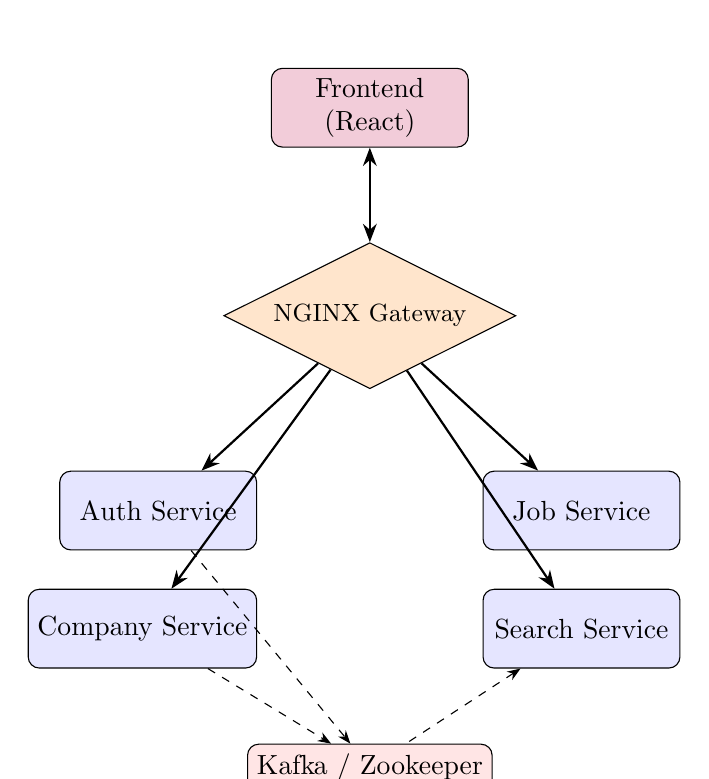
\begin{tikzpicture}[>=Stealth, node distance=1.2cm,
    service/.style={draw, rounded corners, minimum width=2.5cm, minimum height=1cm, align=center, fill=blue!10},
    gate/.style={draw, diamond, aspect=2, fill=orange!20, font=\small},
    db/.style={draw, cylinder, shape border rotate=90, minimum width=1.5cm, minimum height=1.5cm, fill=green!10},
    msg/.style={draw, rounded corners, minimum width=3cm, fill=red!10}
]

% Nodes
\node[service, fill=purple!20] (fe) {Frontend\\(React)};
\node[gate, below=of fe] (gateway) {NGINX Gateway};

\node[service, below left=1.5cm and 0.5cm of gateway] (auth) {Auth Service};
\node[service, below left=3cm and 0.5cm of gateway] (company) {Company Service};
\node[service, below right=1.5cm and 0.5cm of gateway] (job) {Job Service};
\node[service, below right=3cm and 0.5cm of gateway] (search) {Search Service};

\node[msg, below=4.5cm of gateway] (kafka) {Kafka / Zookeeper};

% Connections
\draw[<->, thick] (fe) -- (gateway);
\draw[->, thick] (gateway) -- (auth);
\draw[->, thick] (gateway) -- (company);
\draw[->, thick] (gateway) -- (job);
\draw[->, thick] (gateway) -- (search);

\draw[->, dashed] (auth) -- (kafka);
\draw[->, dashed] (company) -- (kafka);
\draw[<-, dashed] (search) -- (kafka);

\end{tikzpicture}
\caption{DevVision Microservices Architecture}
\end{figure}

\newpage

% -----------------------------------------------------------
\chapter{Data Model}
The following table outlines the core data entities and their primary attributes.

\section{Entity Definitions}
\begin{singlespacing}
\begin{longtable}{@{} p{3cm} p{6cm} p{6cm} @{}}
\caption{System Data Models} \\
\toprule
\textbf{Entity} & \textbf{Attributes} & \textbf{Description} \\
\midrule
\endhead
\textbf{User} & email, password, role & Basic authentication data stored in the Auth Service. \\
\midrule
\textbf{Company} & name, country, city, address, phone & Extended profile details linked to a User ID. \\
\midrule
\textbf{Job} & title, description, skills, salary, status & Work opportunities created by premium companies. \\
\midrule
\textbf{Application} & jobId, applicantId, resume, status & Represents a candidate's interest in a specific job. \\
\midrule
\textbf{Applicant} & name, headline, skills, summary & Searchable profile record used by the Search service. \\
\bottomrule
\end{longtable}
\end{singlespacing}

\newpage

% -----------------------------------------------------------
\chapter{API Documentation}

\section{Endpoint Summary}

\subsection{Authentication Service}
\begin{itemize}
    \item \texttt{POST /auth/signup}: Primary registration for company users.
    \item \texttt{POST /auth/signin}: Secure login returning JWT payloads.
    \item \texttt{POST /auth/refresh-token}: Token rotation for persistent sessions.
\end{itemize}

\subsection{Company Service}
\begin{itemize}
    \item \texttt{GET /companies/:id}: Retrieve current profile data.
    \item \texttt{PUT /companies/:id}: Update profile and propagate via Kafka.
\end{itemize}

\subsection{Job Service}
\begin{itemize}
    \item \texttt{POST /jobs}: Create a new job vacancy.
    \item \texttt{GET /jobs/company/:id}: Fetch all jobs belonging to the requester.
    \item \texttt{POST /jobs/:id/apply}: Submit an external applicant's resume.
\end{itemize}

\subsection{Search Service}
\begin{itemize}
    \item \texttt{GET /search/applicants?q=...}: High-speed query engine for talent scouting.
\end{itemize}

\section{The NGINX Gateway}
The gateway logic is crucial for masking the complexity of the backend. It maps incoming traffic on port \texttt{8080} to the internal microservice cluster:
\begin{itemize}
    \item Routes ending in \texttt{/api/auth/*} $\rightarrow$ \texttt{http://auth-service:3000}
    \item Routes ending in \texttt{/api/companies/*} $\rightarrow$ \texttt{http://company-service:3000}
\end{itemize}

\newpage

% -----------------------------------------------------------
% -----------------------------------------------------------
\chapter{Project Compliance and Feature Implementation}

This chapter details the specific requirements fulfilled by the DevVision Job Manager subsystem, organized by complexity and architectural type.

\section{Functional Requirements Quota}
The system fulfills the target quota of \textbf{4 Simplex, 5 Medium, and 3 Ultimo} requirements.

\begin{singlespacing}
\begin{longtable}{@{} l l p{8cm} @{}}
\caption{Implemented Functional Requirements} \\
\toprule
\textbf{Category} & \textbf{ID} & \textbf{Implemented Feature} \\
\midrule
\endhead
\textbf{Simplex} & 1.1.1 & Core user registration fields (Email, Pwd). \\
                 & 1.1.2 & Unique email enforcement during signup. \\
                 & 2.1.2 & Token-based authentication (JWT). \\
                 & 3.1.1 & Company profile editing capabilities. \\
                 & 4.1.1 & Standard job posting functionality. \\
\midrule
\textbf{Medium} & 1.2.1 & Advanced Password Strength validation (Regex). \\
                & 1.2.2 & Email syntax validation and normalization. \\
                & 2.2.1 & JWE Upgrade for secure payload encryption. \\
                & 4.2.1 & Skill tagging for job Categorization. \\
                & 5.2.1 & Full-text search (FTS) for applicants. \\
                & 5.2.4 & High-performance responsive search results. \\
\midrule
\textbf{Ultimo} & 2.3.3 & Refresh-token rotation and session management. \\
                & 4.3.1 & \textbf{Kafka Propagation}: Real-time profile/country updates. \\
                & 4.3.2 & CV and Cover Letter file storage and display. \\
\bottomrule
\end{longtable}
\end{singlespacing}

\section{Technical and Architectural Compliance}
The project adheres to the strict architectural constraints defined for the project.

\subsection{API Integration and Provision}
\begin{itemize}
    \item \textbf{API Integration}: The \texttt{JobApplication} workflow in the \textit{Job Service} utilizes a mock internal data service for applicant validation, satisfying the 1-out-of-3 API integration rule.
    \item \textbf{API Provision}: The \texttt{Company Service} provides the 1st choice provision mechanism by publishing event-driven data to \textbf{Kafka}, allowing external microservices to consume profile updates autonomously.
\end{itemize}

\subsection{Architecture and Deployment}
\begin{itemize}
    \item \textbf{Complete Ultimo Architecture}: The system is fully decentralized into four discrete microservices (\textit{Auth, Company, Job, Search}) and utilizes a dedicated Message Broker (Kafka) for inter-service communication.
    \item \textbf{Medium Backend}: Each microservice implements a strict \textbf{Repository Pattern} (as per A.1.2/A.2.2), abstracting all Mongoose database interactions behind a specialized repository layer.
    \item \textbf{Medium Deployment}: The entire lifecycle is managed via a single \textit{Docker Compose} configuration, including the gateway, database, messaging, and application services.
\end{itemize}

\chapter{Deployment and Orchestration}

\section{Containerization}
The entire DevVision ecosystem is containerized using \textbf{Docker}. This ensures that the development, staging, and production environments are identical.

\section{Orchestration with Docker Compose}
A single command orchestrates the lifecycle of all services, including dependencies like Redis and Kafka.

\begin{lstlisting}[language=bash, caption={Deploying the System}]
# Build all images and start containers in detached mode
docker compose up -d --build
\end{lstlisting}

\section{Environment Configuration}
Each service is configured via environment variables, pointing to the shared \textit{MongoDB Atlas} cluster and the internal \textit{Kafka} bootstrap servers.

\chapter{Conclusion}
The DevVision project serves as a comprehensive demonstration of scalable system design. By leveraging microservices, asynchronous messaging, and the repository pattern, we have built a platform that is both maintainable and performant.

\end{document}
